\chapter{Implementation and Testing}
\subsection{Implementation Environment}
\subsubsection{Programming Tools:}
Unity Hub \& Unity Engine were used as primary development tools for the game, where game assets, scenes, physics and animations were handled.Visual Studio Community version was employed for scripting and debugging C\# scripts.
The Unity Asset Store leveraged for acquiring free assets, such as character models, environments, and particle effects to enrich the game's visuals and functionalities.
\subsubsection{Repository Setup \& Version Control:}
Git \& GitHub was used as a version control system to track changes and maintain backups of the project.
\subsubsection{Integration:}
The game integrated multiple components like 3D models from the Asset Store, sound assets, and physics libraries within Unity.
Testing \& Debugging was performed through Visual Studio and Unity’s built-in play testing features.
In Unity, the Play Mode allows you to run the game within the Unity Editor itself. This lets you test the game in real time without needing to build and deploy it to a separate platform.
\subsubsection{Team Development Tools}
To make a plan and for easy management of the project, Trello was used.
\subsection{High Level Description Major Program Modules:}
The high-level program modules consist of the main classes that play a crucial role in the core functionality of the system. These key classes manage essential operations such as game logic, user interaction, and overall flow. While there are additional supporting classes that handle specific tasks (e.g., utilities, minor features)..
\subsection{PlayerController.cs}
\begin{itemize}
	\item \textbf{Description:} This module handles player input, movements, and interactions with the environment. 
	It defines how the character moves in response to user input and interacts with in-game objects.
	
	\item \textbf{Data Tables:} Keeps track of player stats such as health, position, inventory, and weapons.
	\item \textbf{Error Handling:} Includes checks for invalid inputs and collision detection to avoid bugs related to character movement.
\end{itemize}
\subsection{EnemyAI.cs}
\begin{itemize}
	\item \textbf{Description:} Controls enemy behavior, including patrol routes, detection of the player, and attack patterns. The enemy reacts when the player enters its detection zone.
	\item \textbf{Data Tables:} Enemy health, position, and state (idle, attack, patrol).
	\item \textbf{Error Handling:} Implements fail-safes to reset enemy states if unexpected behavior occurs, such as getting stuck in the environment.
\end{itemize}
\subsubsection{InventorySystem.cs}
\begin{itemize}
	\item \textbf{Description:} Manages the player’s inventory, including adding, removing, and using items. Links the player's interactions with the in-game shop.
	\item \textbf{Data Tables:} Item IDs, quantities, and descriptions.
	\item \textbf{Error Handling}: Prevents overflow (carrying more items than allowed) and invalid item usages.
\end{itemize}
\subsection{UIManager.cs}

\begin{itemize}
	\item \textbf{Description}: Manages the UI elements like the HUD, menus, and in-game notifications. Ensures that UI elements update dynamically during gameplay (health bars, ammo count).
	\item \textbf{Data Tables:} UI elements’ visibility, text, and buttons.
	\item \textbf{Error Handling:} Detects and fixes null references in UI elements to prevent crashes.
\end{itemize}

\subsection{ Design of Implemented Module Structure:}
Below is the diagram for Module Structure
\\
\\
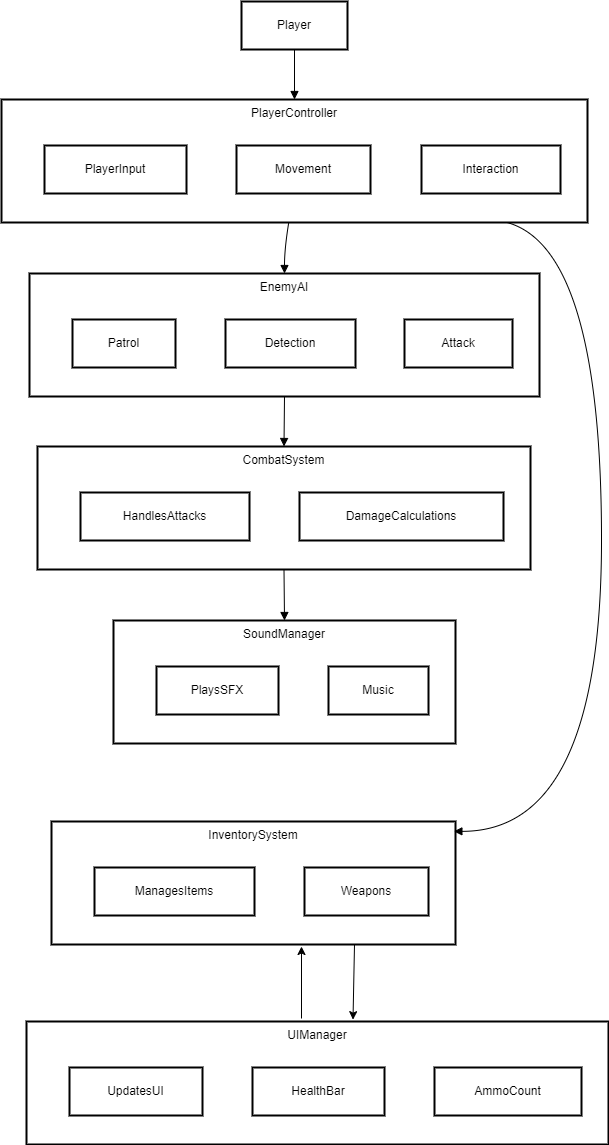
\includegraphics[width=16cm,height=18cm]{C://Users/PMLS/Desktop/Thesis/Latex Thesis/Design of Implemented Module Structure.png}
\\
\\
\textbf{PlayerController}:
\begin{itemize}
	\item Manages user input, character movement, and player interactions with the environment.
	\item Links to \texttt{InventorySystem} to update inventory when picking up or using items.
	\item Also links to \texttt{UIManager} to ensure the user interface reflects player status (e.g., health, ammo).
\end{itemize}

\textbf{InventorySystem}:
\begin{itemize}
	\item Manages items and weapons.
	\item Communicates with \texttt{UIManager} to display the correct items and quantities on the screen.
\end{itemize}

\textbf{UIManager}:
\begin{itemize}
	\item Updates the user interface dynamically based on player actions and status changes.
\end{itemize}

\textbf{EnemyAI}:
\begin{itemize}
	\item Handles enemy movement, patrol behavior, and attacks.
	\item Communicates with the \texttt{CombatSystem} to calculate and apply damage when the player and enemy interact.
\end{itemize}

\textbf{CombatSystem}:
\begin{itemize}
	\item Coordinates attack logic and damage calculations between the player and enemies.
\end{itemize}

\textbf{SoundManager}:
\begin{itemize}
	\item Plays sound effects (SFX) and music based on game events such as attacks, item pickups, or changes in player state.
	\end{itemize}
	

\subsection{Test Strategies}
The testing approach employed during the game development process was centred on both automated and manual testing in order to guarantee seamless gaming, error-free operation, and an intuitive user experience. Important phases of testing were:

\begin{itemize}
	\item \textbf{Unit Testing:}
	Every essential feature, such as inventory management, adversary AI behaviour, and player controls, was tested separately.
	The behaviour of scripts such as PlayerController.cs and EnemyAI.cs, which handle erroneous input, boundary conditions, and stress testing, was verified by testing.
	\item \textbf{Integration Testing:}
	Each module's ability to function alone was checked, and then it was examined how well it interacted with the others (for example, connecting the PlayerController to the InventorySystem and UIManager).
	\item \textbf{Play Testing (Manual Testing):}
	Frequent playtests were carried out to find flaws that could only be discovered during runtime, difficulty balancing, and unexpected enemy AI behaviours.
	Playtests also paid attention to the user experience.
	\item \textbf{Performance Testing:}
	Load testing was done to ensure the game performed well on a range of devices, testing for frame rate drops, memory usage, and lag.
	The game’s performance was checked with higher numbers of enemies, effects, and environmental details to ensure it could handle complex scenarios without performance degradation.
	\item \textbf{Regression Testing:}
	Every time a new feature or bug fix was introduced, regression testing ensured that previously working features were still functioning as intended.
	The version control system (GitHub) was used to track and merge changes, helping avoid conflicts that could introduce bugs. Several times Git has helped to travel back in time and fix issues in code.
\end{itemize}

\subsection{White Box Testing}
\subsubsection{Unit Testing the Individual Classes and Methods:} 
Software testing that involves testing individual program modules or components separately is known as unit testing \cite{fowler_unit_test}. A function, method, or class is the smallest tested component that makes up a "unit" in an application. Unit testing makes sure that every single portion of the code runs correctly without interference from outside sources.
\begin{itemize}
	\item  \textbf{AI.cs Unit Test:}
	\\
	AI behavior based on conditions (e.g., proximity to the player, attack conditions).
	\begin{lstlisting}
[Test]
public void Test_AI_Movement()
{
	// Arrange
	AI ai = new AI();
	ai.followSnds = new AudioClip[1]; // Assuming AI has audio clips for movement sound
	// Act
	ai.Move();  // Call the movement function
	// Assert
	// Add assertions depending on the conditions of Move, like if it moves to the correct destination
}
	\end{lstlisting}
	\item  \textbf{CharacterDamage.cs Unit Test:}
	\\
	This script involves handling damage to NPCs and tracking hit points. Important methods of this class include taking damage and removing the character upon death.
	\item \textbf{TakeDamage():} How the character's hit points are reduced.
	\item \textbf{Death event():} Whether the body is removed when health reaches zero.
	\begin{lstlisting}
		[Test]
		public void Test_Character_TakesDamage()
		{
			// Arrange
			CharacterDamage character = new CharacterDamage();
			character.hitPoints = 100f;
			// Act
			character.TakeDamage(30f);  // Simulate 30 points of damage
			// Assert
			Assert.AreEqual(70f, character.hitPoints, "Character should have 70 hit points left after taking 30 damage.");
		}
		[Test]
		public void Test_Character_Dies_When_Health_Depletes()
		{
			// Arrange
			CharacterDamage character = new CharacterDamage();
			character.hitPoints = 50f;
			// Act
			character.TakeDamage(60f);  // Damage exceeds current hit points
			// Assert
			Assert.AreEqual(0f, character.hitPoints, "Character hit points should not go below zero.");
			// Additional checks for death behavior can be added, such as checking if the onDie event is called.
		}
	\end{lstlisting}
	\item \textbf{ MoveTrigger.cs Unit Test:}
	\\
	This script manages NPC movement triggers. It detects when an NPC (Non-Player Character) should move or rotate towards a target.
	\begin{lstlisting}
		[Test]
		public void Test_NPC_Moves_On_Trigger()
		{   // Arrange
			MoveTrigger moveTrigger = new MoveTrigger();
			NPC npc = new NPC(); // Assuming an NPC class exists and npcToMove refers to it
			moveTrigger.npcToMove = npc;
			// Act
			moveTrigger.OnTriggerEnter();  // Simulate entering a movement trigger
			// Assert
			Assert.IsTrue(npc.followed, "NPC should follow the player when the move trigger is activated.");
		}
	\end{lstlisting}
	\item \textbf{RemoveBody.cs Unit Testing:}
	\\
	This script is responsible for removing NPC bodies after a certain time (bodyStayTime) and removal of weapons.
	\begin{lstlisting}
	[Test]
	public void Test_Body_Removed_After_Delay()
	{   // Arrange
		RemoveBody removeBody = new RemoveBody();
		removeBody.bodyStayTime = 5f;  // Set stay time to 5 seconds for test purposes
		GameObject body = new GameObject();
		// Act
		removeBody.Start();  // Start timer
		removeBody.FixedUpdate();  // Simulate time passing
		// Assert
		// Check if the body is removed after the specified delay (this would require simulating time)
	}
	\end{lstlisting}
\end{itemize}

\subsection{Integration Testing}
In integration testing we check how the code for different functionalities integrates with other functionalities. After manual testing of each and every feature the project is working fully and the code is free from any large scale bugs.

\begin{itemize}
	\item  \textbf{Full Integration Test: Combining AI, CharacterDamage, and RemoveBody}
	This comprehensive test checks the full interaction: AI attacking the player, the player taking damage and dying, and the body being removed.
	\begin{lstlisting}
		using NUnit.Framework;
		using UnityEngine;
		using System.Collections;
		public class FullIntegrationTest : MonoBehaviour
		{   private AI ai;
			private CharacterDamage player;
			private RemoveBody removeBody;
			[SetUp]
			public void Setup()
			{   // Setup AI, player, and remove body in the scene
				GameObject aiObject = new GameObject();
				ai = aiObject.AddComponent<AI>();
				GameObject playerObject = new GameObject();
				player = playerObject.AddComponent<CharacterDamage>();
				removeBody = playerObject.AddComponent<RemoveBody>();
				// Assign player to AI and configure settings
				ai.player = player;
				ai.playerProximity = 5f;  // AI will attack within 5 units
				player.hitPoints = 100f;  // Player starts with 100 hit points
				removeBody.bodyStayTime = 2f;  // Body will be removed after 2 seconds
			}
			[UnityTest]  // Use UnityTest for time-based operations
			public IEnumerator Test_AI_Attacks_Player_And_Body_Removed()
			{   // Simulate AI getting close to the player and attacking
				ai.transform.position = new Vector3(0, 0, 0);
				player.transform.position = new Vector3(3, 0, 0);  // Player within attack range
				ai.Update();  // Update AI to check proximity and attack
				// Assert: Player took damage
				Assert.Less(player.hitPoints, 100f, "Player should take damage from AI attack.");
				// Simulate player dying
				player.TakeDamage(150f);  // Lethal damage to player
				// Wait for bodyStayTime to pass
				yield return new WaitForSeconds(removeBody.bodyStayTime);
				// Assert: Player's body is removed
				Assert.IsNull(player.gameObject, "Player's body should be removed after bodyStayTime.");
			}
		}
	\end{lstlisting}
	
	\item  \textbf{Explanation}
	To make sure that various game elements—such as AI, player health, and movement triggers—interact as intended during actual game play, Unity integration testing is essential. The tests offered confirm how certain parts function together:
	\begin{enumerate}
		\item \textbf{AI attacking the player:} AI that attacks the player makes sure that damage-dealing and proximity detection work as they should.
		\item \textbf{Character death and body removal:} Game realism is increased by character death and body removal tests that determine whether the body object is properly removed after a predetermined amount of time.
		\item \textbf{NPC movement triggers:} NPC movement triggers verify whether the NPC responds to triggers correctly by moving to designated positions.
		\item \textbf{Full Integration Test:} A full integration test simulates every step of the gaming flow, from AI attack to player death and body removal, by combining several different components.\\
		These integration tests guarantee that the game mechanics function as a cohesive unit by covering crucial script-to-script interactions. These tests are adaptable to the unique gameplay situations and game features.
	\end{enumerate}
\end{itemize}
\subsection{Black Box Testing}
Black box testing is a type of software testing where the tester assesses an application's functioning without looking inside its core components or operations.
\subsubsection{Techniques Used in Black Box Testing:}
\begin{itemize}
	\item \textbf{Equivalence Partitioning:} Equivalence Partitioning splits input data into segments that are valid and invalid in order to minimize the number of test cases.
	\item \textbf{Boundary Value Analysis:} Boundary Value Analysis tests the limits of the partitions, including the points directly below, at, and above the boundaries.
	\item \textbf{Decision Table Testing:} Decision Table Testing represents combinations of inputs and their matching outputs using a table.
	\item \textbf{State Transition Testing:} State Transition Testing evaluates the system's ability to change states in response to input circumstances.
	\item \textbf{Use Case Testing:} Use Case Testing uses use cases and user scenarios to validate the functionality.
\end{itemize}
\begin{table}[ht]
	\centering
	\resizebox{1.1\textwidth}{!}{
	\begin{tabular}{|c|c|c|c|c|}
		\hline
		\textbf{Test Case ID} & \textbf{Component} & \textbf{Input} & \textbf{Expected Output} & \textbf{Result} \\
		\hline
		TC1 & AI.cs & Player is within proximity of AI & AI should attack the player and reduce the player’s hit points. & Pass \\
		\hline
		TC2 & AI.cs & Player is outside AI proximity & AI should not attack the player, and player’s hit points remain unchanged. & Pass \\
		\hline
		TC3 & CharacterDamage.cs & Player takes 30 damage when hit & Player’s hit points should reduce by 30 from the initial value. & Pass \\
		\hline
		TC4 & CharacterDamage.cs & Player takes damage exceeding health & Player’s health should not drop below zero, and the death event should trigger. & Pass \\
		\hline
		TC5 & CharacterDamage.cs & Player is dealt no damage & Player’s hit points should remain the same. & Pass \\
		\hline
		TC6 & MoveTrigger.cs & NPC enters trigger zone & NPC should move to the designated location defined in the \texttt{movePosition}. & Pass \\
		\hline
		TC7 & MoveTrigger.cs & NPC does not enter trigger zone & NPC should remain at its original position. & Pass \\
		\hline
		TC8 & RemoveBody.cs & Character dies and \texttt{bodyStayTime} is set & Character’s body should be removed after the \texttt{bodyStayTime} passes. & Pass \\
		\hline
		TC9 & RemoveBody.cs & \texttt{bodyStayTime} set to 0 & Character’s body should be removed immediately after death. & Pass \\
		\hline
		TC10 & RemoveBody.cs & Player remains alive & Character’s body should not be removed as the player is still alive. & Pass \\
		\hline
		TC11 & AI + CharacterDamage (Integration Test) & Player is within AI range, and AI attacks & Player’s hit points should reduce, and after enough damage, the player should die. & Pass \\
		\hline
		TC12 & AI + MoveTrigger (Integration Test) & AI reaches target position via trigger zone & AI should correctly navigate and stop at the target position defined by the trigger. & Pass \\
		\hline
		TC13 & Full Integration (AI + CharacterDamage + RemoveBody) & Player is killed by AI, \texttt{bodyStayTime} triggers & Player’s health should drop to zero, triggering death, and the body should be removed after a delay. & Pass \\
		\hline
	\end{tabular}
}
	\caption{Black-box testing results for game scripts}
\end{table}
\subsection{Usability Report For Proximity Assault}
\begin{enumerate}
	\item \textbf{Title Page`}
	\begin{itemize}
		\item \textbf{Title:} Usability Report for Proximity Assault
		\item \textbf{Project:} First-Person Shooting Game
		\item \textbf{Prepared By:} Muhammad Atif
	\end{itemize}
	\item \textbf{Executive Summary}
	The purpose of this usability test was to assess the player's experience in the game, in which terrorists have taken over a facility and are getting ready to produce nuclear weapons. The player's goal is to use a variety of weaponry to destroy every enemy so that a group of scientists can disassemble the nuclear apparatus.
	\item \textbf{Introduction}
	\begin{itemize}
		\item \textbf{Purpose:} The goal of the test was to find problems with the controls, navigation, and degree of difficulty of the gaming experience.
		\item \textbf{Scope:} The first two stages of the game, the weapon swapping mechanism, enemy encounters, and mission objectives.
	\end{itemize}
	\item \textbf{Methodology}
	\begin{itemize}
		\item \textbf{Participants:} 4 participants, aged 18-25 with a mix of gaming experience.
		\item \textbf{Environment:} The test was conducted on the users phones.
		\item \textbf{Task:} The user navigate through the scenes, switched weapons and tried different weapons.
		\item \textbf{Data Collection:} Data was collected through screen recording.
	\end{itemize}
	\item \textbf{Results}
	\begin{itemize}
		\item \textbf{Task Completion Rate}
		\begin{table}[h]
			\centering
			\caption{Task Completion Rates and Findings}
			\begin{tabular}{|l|c|c|c|}
				\hline
				\textbf{Task} & \textbf{Success Rate} & \textbf{Average Time on Task} & \textbf{Error Rate} \\ \hline
				Navigate through the facility & 90\% & 4 minutes & 5\% \\ \hline
				Switch weapons and eliminate enemies & 75\% & 6 minutes & 20\% \\ \hline
			\end{tabular}
		\end{table}
	\item \textbf{Usability Issues:}
		\item \textbf{Weapon Switching Difficulty:}
	\begin{itemize}
		\item {60\% of players found it difficult to switch between weapons quickly.}
		\item {\textbf{Feedback:} "I couldn't switch weapons fast enough to keep up with the enemies. It was frustrating, especially during intense battles."}
	\end{itemize}
	\item \textbf{Enemy AI Behavior:}
	\begin{itemize}
		\item {Players noted inconsistent enemy AI. Some enemies were too easy, while others felt overpowered.}
		\item {\textbf{Feedback:} "The enemies seemed random in their difficulty. Some stood there doing nothing while others were nearly impossible to beat."}
	\end{itemize}
	\item \textbf{Objective Clarity:}
	\begin{itemize}
		\item {50\% of players had difficulty understanding when and how to protect the scientists during the mission.}
		\item{ \textbf{Feedback:} "I wasn't sure what I was supposed to do after defeating the enemies."}
	\end{itemize}
	\end{itemize}
	\item \textbf{Analysis}
	\begin{itemize}
		\item \textbf{Weapon Switching Mechanism:}
		The present weapon swapping system is clumsy and takes away from the intense fighting.
		\item \textbf{Enemy AI:}
		Players became frustrated with the inconsistent behaviour of the enemies, which decreased their level of enjoyment with the game overall.
		\item \textbf{Mission Objectives:}
		The lack of clarity in communicating objectives resulted in a decrease in task success rates and confusion.
	\end{itemize}
		\item \textbf{Recommendations}
	\begin{itemize}
		\item \textbf{Improve Weapon Switching}

		\item \textbf{Enhance AI Behavior}
		\item \textbf{Clearer Mission Guidance}
	\end{itemize}
	\item \textbf{Conclusion}
	Overall, the results of the usability test indicated that while participants found the concept and ambiance of the game engaging, they found certain elements difficult to grasp, such as switching between weapons and mission objectives.
\end{enumerate}














